\documentclass[xcolor=dvipsnames]{beamer}
\usetheme{Boadilla}

\definecolor{HKARedPrim}{RGB}{215, 34, 5}
\definecolor{HFUGreenSec}{RGB}{0, 132, 77}
\definecolor{HFUGrey}{RGB}{218, 220, 220}
\definecolor{HFUAnthr}{RGB}{112, 113, 115}
\usecolortheme[named=HKARedPrim]{structure}
\setbeamertemplate{section in toc}[circle]
\setbeamertemplate{subsection in toc}[square]

\setbeamertemplate{frametitle}{\vspace{0.9em}\textbf{\insertframetitle}}

\usepackage[T1]{fontenc}
\usepackage[ngerman]{babel}
\usepackage{graphicx}
\usepackage{eso-pic}

\title[PA2]{\textbf{Seminararbeit}}
\subtitle{Dynamische Programmanalysen für nebenläufige Programme - Data Race Prediction mit TSan}
\author[Frank Ling]{
\includegraphics[trim={1230px 0 0 0}, clip, scale=0.1]{pics/HKA_Logo_Logoleiste_RGB.png}\\Frank Ling}
\date{13. Juni 2023}
\setbeamertemplate{itemize item}{$\circ$}

\begin{document}
	
	\frame{\titlepage}
	
	\newcommand\AtPagemyUpperLeft[1]{\AtPageLowerLeft{%
			\put(\LenToUnit{0.6\paperwidth},\LenToUnit{0.86\paperheight}){#1}}}
	\AddToShipoutPictureFG{
		\AtPagemyUpperLeft{{
\includegraphics[scale=0.06]{pics/HKA_Logo_Logoleiste_RGB.png}}}
	}%
	
	\frame{
		\frametitle{Table of contents}
		\tableofcontents
	}
	
	\section{Introduction}
	\frame{
		\frametitle{Introduction}
		\begin{columns}
			\begin{column}{0.5\textwidth}
				\begin{itemize}
					\item What are data races?
					\item Why fix data races?
					\item How to detect data races?
					\item show code snippets and corresponding traces
				\end{itemize}
			\end{column}
			\begin{column}{0.5\textwidth}
				\centering
				\begin{figure}
					\includegraphics[scale=0.28]{example-image}
				\end{figure}
				$\big\Downarrow$
				\begin{figure}
					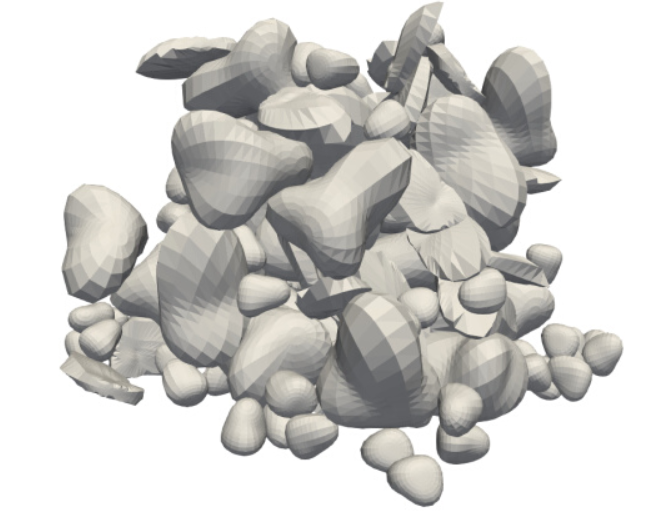
\includegraphics[scale=0.25]{pics/packing.png}
					\newline
					\tiny Output: Packing
				\end{figure}
			\end{column}
		\end{columns}
	}

	\frame{
		\frametitle{Happens-before relation}
		\begin{columns}
			\begin{column}{0.5\textwidth}
				\begin{itemize}
					\item Lamport's HB relation
				\end{itemize}
			\end{column}
			\begin{column}{0.5\textwidth}
				\centering
				\begin{figure}
					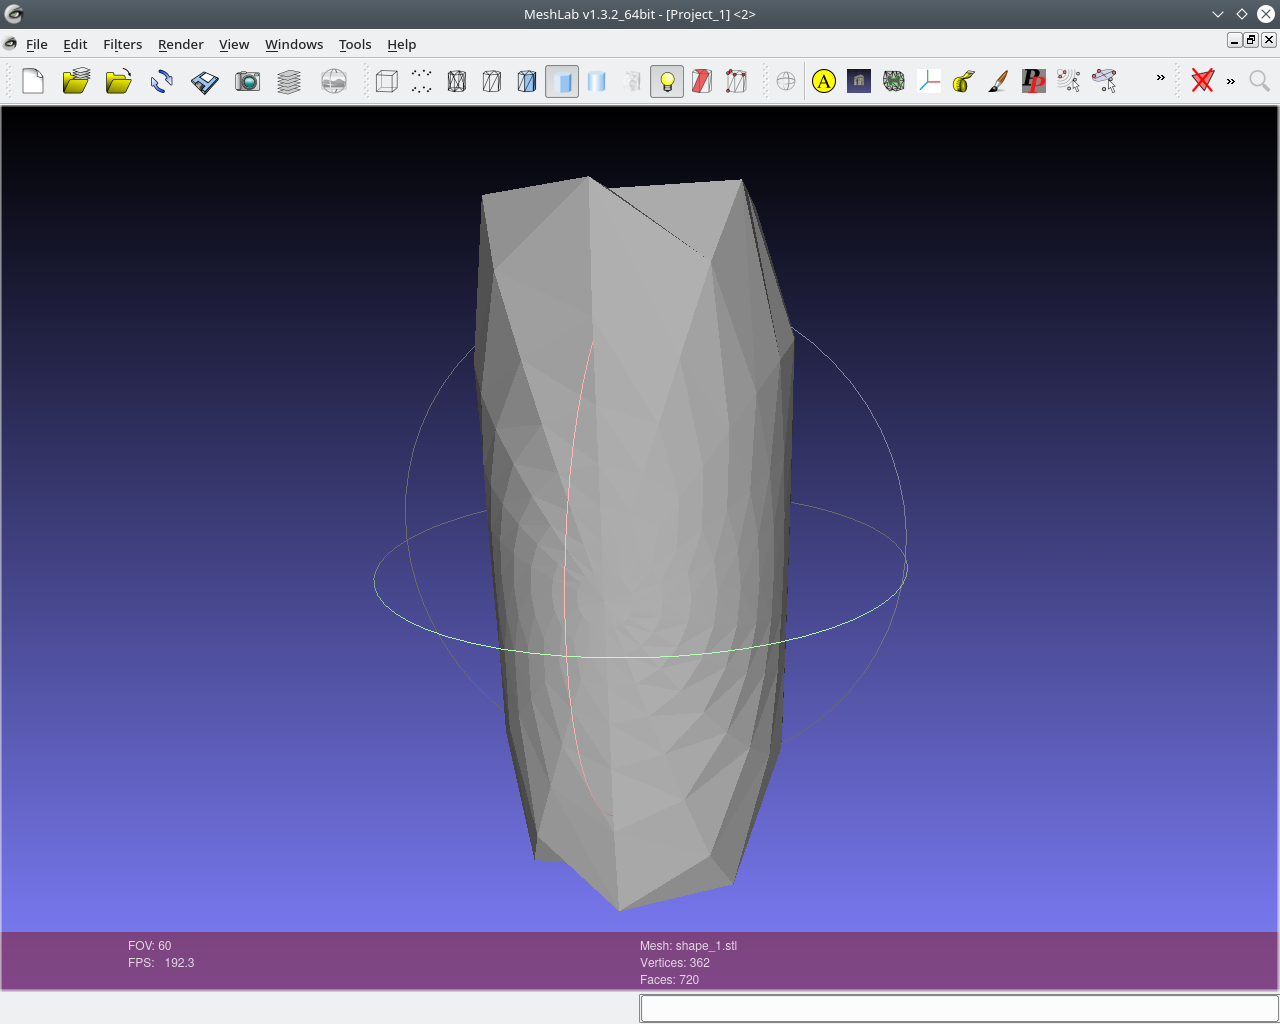
\includegraphics[scale=0.12]{pics/Screenshot_20221115_151950.png}
				\end{figure}
				\begin{figure}
					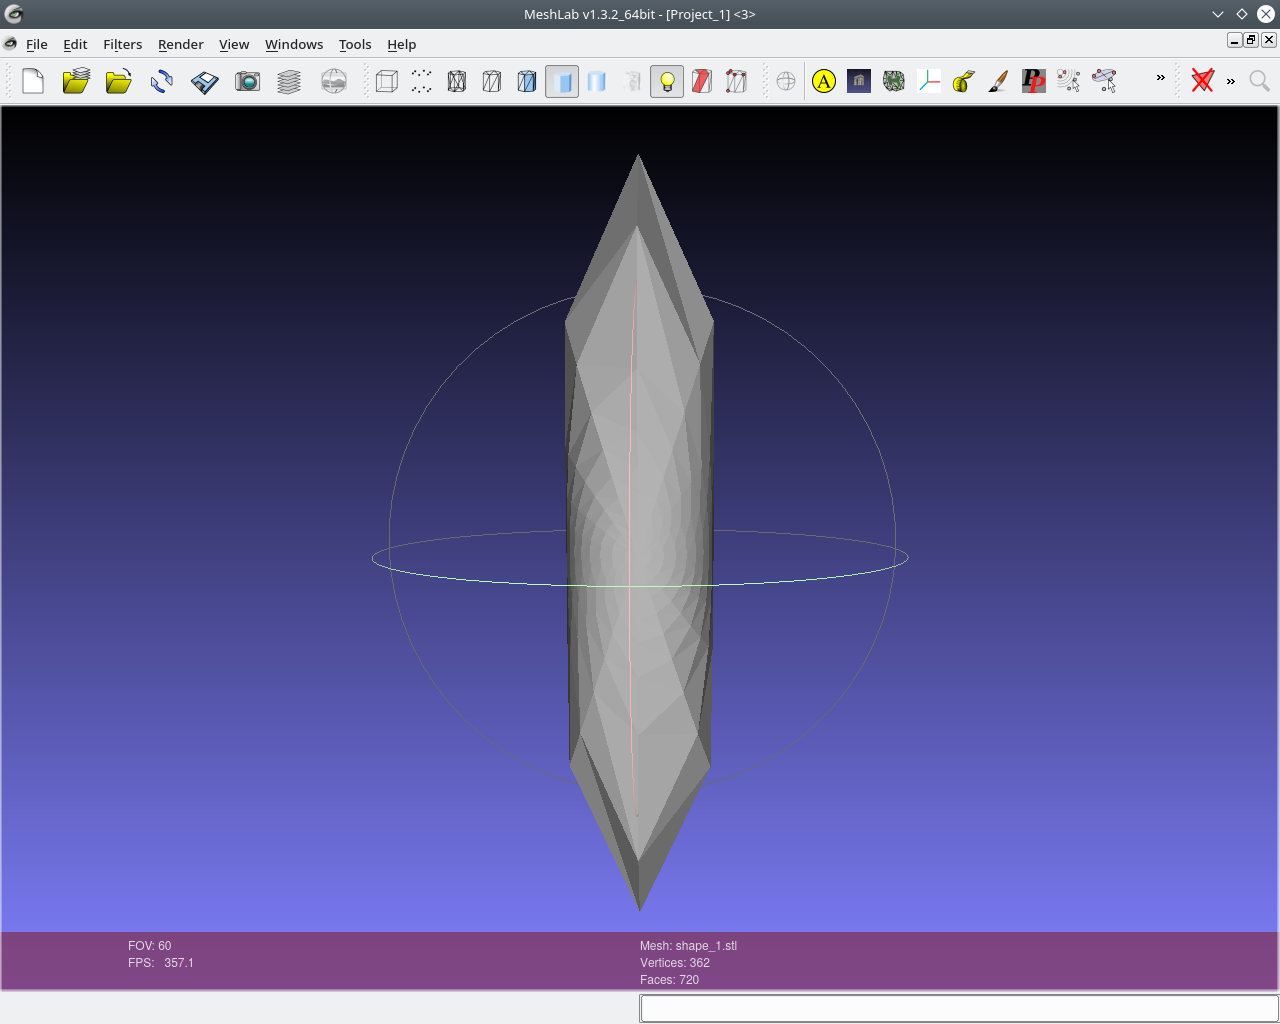
\includegraphics[scale=0.12]{pics/Screenshot_20221115_152310.png}
				\end{figure}
			\end{column}
		\end{columns}
	}
	
	\section{FastTrack}
	\frame{
		\frametitle{FastTrack}
	}
	
	\section{TSan}
	\frame{
		\frametitle{TSan V2}
	}
	
	\section{Conclusion}
	\frame{
		\frametitle{Conclusion}
	}
	
\end{document}
